%\documentclass[12pt, a4paper, oneside, openany]{Thesis}
\documentclass[12pt, a4paper, oneside, openany]{Thesis} % Paper size, default font size and one-sided paper
\usepackage{wrapfig}
\usepackage{lscape}
\usepackage{rotating}
\usepackage{graphicx}
\usepackage{caption}
\usepackage{comment}
\usepackage{afterpage}
\usepackage{multirow}
\usepackage{multicol}
\usepackage{cleveref}
\usepackage{rotating}
\usepackage{adjustbox}
\usepackage[ruled,vlined]{algorithm2e}
\usepackage{amsmath,amssymb,amsfonts}
\usepackage{algorithmic}
\usepackage{graphicx}
\usepackage{textcomp}
\usepackage{xcolor}
\usepackage{balance}
\usepackage{enumitem}
\usepackage{setspace}
\usepackage{listings}
\usepackage{color}
%\usepackage{subcaption}
\usepackage{subfig}
\usepackage{cancel}
\usepackage[many]{tcolorbox}
\usepackage[dmyyyy]{datetime}
\usepackage{changepage}
\usepackage{colortbl}
%\usepackage{pdfpages}
\usepackage[acronym]{glossaries}

\usepackage{acro}

\hypersetup{
    colorlinks=true,
    allcolors=black
}

\makeglossaries


\newcommand\myemptypage{
    \null
    \thispagestyle{empty}
    \addtocounter{page}{-1}
    \newpage
    }
\usepackage{amssymb}

\usepackage{amsmath}
\DeclareMathOperator*{\argmax}{arg\,max}
\DeclareMathOperator*{\argmin}{arg\,min}
\usepackage{mathtools}
\DeclarePairedDelimiter\ceil{\lceil}{\rceil}
\DeclarePairedDelimiter\floor{\lfloor}{\rfloor}

\usepackage[tikz]{bclogo}
\usepackage{tikz}
\usetikzlibrary{calc, shapes.geometric, arrows}
\tikzstyle{arrow} = [thick,->,>=stealth]
\usetikzlibrary{backgrounds}

\usepackage{placeins}



\renewcommand{\dateseparator}{.}
%\usepackage[width=14cm, left=3cm]{geometry}

% prints author names as small caps


%\usepackage{subcaption} %incompatible with subfig
\graphicspath{{Pictures/}} % Specifies the directory where pictures are stored
\usepackage[square, numbers]{natbib} % Use the natbib reference package - read up on this to edit the reference style; if you want text (e.g. Smith et al., 2012) for the in-text references (instead of numbers), remove 'numbers' v
%\bibliographystyle{abbrvnat}
%\setcitestyle{authoryear,open={((},close={))}}
\hypersetup{urlcolor=black, colorlinks=true} % Colors hyperlinks in blue - change to black if annoyingv`	
\title{Thesis title} % Defines the thesis title - don't touch this
% Linebreak for URLs that are too long for one line
\PassOptionsToPackage{hyphens}{url}\usepackage{hyperref}

\usepackage[utf8]{inputenc}
\usepackage{graphicx}
\usepackage[dmyyyy]{datetime}
\usepackage{setspace}
% netsoft
%\usepackage[linesnumbered,ruled,vlined,resetcount,algochapter]{algorithm2e}

% prevent footnotes from spanning over multiple pages
\interfootnotelinepenalty=10000
%remove redbox
\hypersetup{pdfborder=0 0 0}

% Remove indentation for footnote
\usepackage[hang,flushmargin]{footmisc} 

\renewcommand{\dateseparator}{.}

\input{thesis.sty}

%%%%%%%%%%%%%%%%%%%%%%%%%%%%%%%%%
%%%% Define Titlepage Format
%%%%%%%%%%%%%%%%%%%%%%%%%%%%%%%%%

\makeatletter
\newcommand{\address}[1]{\newcommand{\@address}{#1}}
\newcommand{\institute}[1]{\newcommand{\@institute}{#1}}

\renewcommand{\maketitle}{
	\begin{titlepage}
    \begin{minipage}[t]{0.25\textwidth}
    \vspace{0pt}
    
\includegraphics[width=\linewidth]{logo_teci.png} % <-- Replace with your actual photo file
\end{minipage}
\hfill
\begin{minipage}[t]{0.335\textwidth}
    \vspace{5em}
    
\includegraphics[width=\linewidth]{BTULogo.png} % <-- Replace with your actual photo file
\end{minipage}
\vskip 4em
		\centering
		{\large\noindent\ignorespaces\@institute\par}
        \vskip 4em
        {\LARGE\noindent\ignorespaces \textsc{Bachelor/Master Thesis}\par}\vskip 2.5em
		\noindent\rule{\textwidth}{1pt}%		
		\vspace{0.8\baselineskip}
		{%
			\LARGE%
			\@title%
		}
		\vspace{0.4\baselineskip}
		\noindent\rule{\textwidth}{1pt}        {\large\noindent\ignorespaces\@author\par}\vskip 2.5em
		

		
		\vskip 2em
		
		
		%{\Large\textsc{Studium}\par}\vskip 0.1em
		%{\Large{\vspace{0.4\baselineskip}Doktoratsstudium der Technischen Wissenschaften\\im Dissertationsgebiet Angewandte Informatik}\par}
		
		%\vskip 2em
		
		
		
		\vskip 4em
        \begin{minipage}{\textwidth}
			\flushleft\large
			%\noindent\rule{\columnwidth}{1pt}
			\textsc{Supervisor}\\
			\normalsize
			Name
		\end{minipage}
        \vskip 3em
		\begin{minipage}{0.495\textwidth}
			\flushleft\large
			%\noindent\rule{\columnwidth}{1pt}
			\textsc{1. Examiner}\\
			\normalsize
			Name
		\end{minipage}
		\begin{minipage}{0.495\textwidth}
			\flushright\large
			%\noindent\rule{\columnwidth}{1pt}
			\textsc{2. Examiner}\\
			\normalsize
			Name
		\end{minipage}
		\vskip 3em
		{\normalsize\noindent\ignorespaces\@address, \@date}
	\end{titlepage}
}
\makeatother




\newacronym{cpu}{CPU}{Central Processing Unit}
\newacronym{ml}{ML}{Machine Learning}
\newacronym{ai}{AI}{Artificial Intelligence}
\newacronym{isa}{ISA}{Instruction Set Architecture}
\newacronym{riscv}{RISC-V}{Reduced Instruction Set Computer V}
\newacronym{soc}{SoC}{System-on-Chip}
\newacronym{hdl}{HDL}{Hardware Description Language}
\newacronym{fpga}{FPGA}{Field-Programmable Gate Array}
\newacronym{asic}{ASIC}{Application-Specific Integrated Circuit}
\newacronym{rtl}{RTL}{Register-Transfer Level}
\newacronym{dse}{DSE}{Design Space Exploration}
\newacronym{ipc}{IPC}{Instructions Per Cycle}
\newacronym{ilp}{ILP}{Instruction-Level Parallelism}
\newacronym{hpm}{HPM}{Hardware Performance Monitor}
\newacronym{mshr}{MSHR}{Miss Status Holding Register}
\newacronym{rob}{ROB}{Reorder Buffer}
\newacronym{uart}{UART}{Universal Asynchronous Receiver-Transmitter}
\newacronym{dram}{DRAM}{Dynamic Random-Access Memory}
\newacronym{sram}{SRAM}{Static Random-Access Memory}
\newacronym{bram}{BRAM}{Block RAM}
\newacronym{lut}{LUT}{Look-Up Table}
\newacronym{ff}{FF}{Flip-Flop}
\newacronym{dsp}{DSP}{Digital Signal Processor}
\newacronym{firrtl}{FIRRTL}{Flexible Intermediate Representation for RTL}
\newacronym{chisel}{Chisel}{Constructing Hardware in a Scala Embedded Language}
\newacronym{boom}{BOOM}{Berkeley Out-of-Order Machine}
\newacronym{csr}{CSR}{Control and Status Register}
\newacronym{sbi}{SBI}{Supervisor Binary Interface}
\newacronym{os}{OS}{Operating System}

\DeclareAcronym{eps}{
  short = $\epsilon$ ,
  long  = epsilon (a small positive quantity),
  class = symbol
}

\DeclareAcronym{avc}{
  short = $\alpha_{vc}$ ,
  long  = alpha value for video coding,
  class = symbol
}



\begin{document}



\author{Student name\\
Immatriculation Number: 123456
}
\institute{
	Brandenburg University of Technology Cottbus - 
Senftenberg\\
Faculty 1 - Institute for Computer Science\\
	Chair for Computer Engineering\\
    Insert Study Program
	
}
\address{Cottbus}
\date{\today}
\maketitle
\thispagestyle{empty}

\makeatletter
\renewcommand*{\NAT@nmfmt}[1]{\textsc{#1}}
\makeatother

% prints author names as small caps


\frontmatter % Use roman page numbering style (i, ii, iii, iv...) for the pre-content pages

\setstretch{1.2} % Line spacing of 1.6 (double line spacing)

% Define the page headers using the FancyHdr package and set up for one-sided printing
\fancyhead{} % Clears all page headers and footers
\rhead{\thepage} % Sets the right side header to show the page number
\lhead{} % Clears the left side page header

\pagestyle{fancy} % Finally, use the "fancy" page style to implement the FancyHdr headers

\newcommand{\HRule}{\rule{\linewidth}{0.5mm}} % New command to make the lines in the title page

% PDF meta-data
\hypersetup{pdftitle={\ttitle}}
\hypersetup{pdfsubject=\subjectname}
\hypersetup{pdfauthor=\authornames}
\hypersetup{pdfkeywords=\keywordnames}

%----------------------------------------------------------------------------------------
%	TITLE PAGE
%----------------------------------------------------------------------------------------
\begin{comment}
\begin{titlepage}
\begin{center}

\HRule \\[0.4cm] % Horizontal line
{\huge \bfseries \ttitle}\\[0.4cm] % Thesis title
\HRule \\[1.5cm] % Horizontal line
 
\large \textit{A thesis submitted in fulfilment of the requirements\\ for the degree of \degreename}\\[0.3cm] % University requirement text
\textit{by}\\[0.4cm]

%\href{http://home.iitk.ac.in/~saiwal}{\authornames}

\vfill
\graphicspath{ {./Figures/} }
\begin{figure}[hb]
  \centering
  \includegraphics[width=0.4\linewidth]{Pictures/aau_circle_logo.jpg}
\end{figure}

\DEPTNAME\\ % Research group name and department name
\textsc{ \UNIVNAME}\\[1.5cm] % University name
\large \today\\[2cm] % Date


\end{center}

\end{titlepage}
\end{comment}
\myemptypage
%\afterpage{\null\newpage}
%\include{blank_page_1}
%\newpage
%\newpage
%\include{title}
%\newpage
%\myemptypage

%----------------------------------------------------------------------------------------
%	DEDICATION
%----------------------------------------------------------------------------------------
%
\setstretch{1.2} % Return the line spacing back to 1.3
%
%\pagestyle{empty} % Page style needs to be empty for this page
%
%\dedicatory{\textit{Dedicated to ...}} % Dedication text
%
%\addtocontents{toc}{\vspace{2em}} % Add a gap in the Contents, for aesthetics
%\newpage


%-------------------------------------------------------------
%	DECLARATION PAGE
%	Your institution may give you a different text to place here
%----------------------------------------------------------------------------------------

%\Declaration{\addtocontents{toc}{\vspace{1em}} % Add a gap in the Contents, for aesthetics

\chapter*{Declaration}
\begin{adjustwidth}{20pt}{20pt}
{	
\singlespacing
The author of this work hereby declares the following:

\begin{enumerate}
  \item This work was completed independently, without outside help and without the use of tools other than those specified. No automated writing aids or artificial intelligence were used in its creation.
  \item Information obtained directly or indirectly from external sources (including electronic sources) is clearly identified as such. Sources used verbatim and in terms of content are cited according to recognized rules of scientific work.
  \item The work has not been submitted in this or a similar form (not even in excerpts) as part of another examination at another university and has not been published.
  \item The author agrees that the work may be checked using a plagiarism detection tool.
  \item Use of AI writing aids (please change as needed): AI writing aids were used exclusively for spell checking, grammar correction, improving formulations, or programming support. 
  All AI-assisted passages are clearly identified and properly cited.
\end{enumerate}

The author is aware that false information and plagiarism can have serious consequences, including the revocation of academic credentials and grades. The author is aware of the responsibility that comes with writing a scientific paper and has completed the work to the best of his/her knowledge and conscience.
	
}

\vskip 12em


\begin{minipage}{\columnwidth}
	\begin{minipage}{0.53\columnwidth}
		%\noindent\rule{\columnwidth}{1pt}
		Student name
	\end{minipage} 
	\begin{minipage}{0.49\columnwidth}
		%\noindent\rule{\columnwidth}{1pt}
		Cottbus, \today
	\end{minipage}
\end{minipage}
\end{adjustwidth}	

\clearpage % Start a new page



%----------------------------------------------------------------------------------------
%	ACKNOWLEDGEMENTS
%----------------------------------------------------------------------------------------

%\setstretch{1.3} % Reset the line-spacing to 1.3 for body text (if it has changed)

\acknowledgements{\addtocontents{toc}{\vspace{1em}} % Add a gap in the Contents, for aesthetics
%\setstretch{1.2}


}
\clearpage % Start a new page

%----------------------------------------------------------------------------------------
%	ABSTRACT PAGE
%----------------------------------------------------------------------------------------

\addtotoc{Abstract - English} % Add the "Abstract" page entry to the Contents

\abstract{\addtocontents{toc}{\vspace{1em}} % Add a gap in the Contents, for aesthetics
\setstretch{1.3}
Write your abstract here. This is a concise summary of your thesis, providing readers with an overview of the content, objectives, methodology, results, and conclusions. Avoid including information not found in the thesis itself and keep the abstract to approximately 100--300 words. It must consist of a single paragraph.
}

\clearpage % Start a new page
%----------------------------------------------------------------------------------------

%----------------------------------------------------------------------------------------
%	ABSTRACT PAGE(German)
%----------------------------------------------------------------------------------------

\addtotoc{Abstract - German} % Add the "Abstract" page entry to the Contents

\abstract{\addtocontents{toc}{\vspace{1em}} % Add a gap in the Contents, for aesthetics
\setstretch{1.3}
Verfassen Sie hier Ihren Abstract. Dabei handelt es sich um eine prägnante Zusammenfassung Ihrer Abschlussarbeit, die Ihren Lesern einen Überblick über den Inhalt, die Ziele, die Methodik, die Ergebnisse und die Schlussfolgerungen der Arbeit bietet. Vermeiden Sie es, Informationen zu geben, die in der Arbeit selbst nicht auftauchen und halten Sie sich an eine Länge von ca. 100-300 Wörtern. Der Abstract muss aus einem einzigen Absatz bestehen.
}

\clearpage % Start a new page
%----------------------------------------------------------------------------------------


%	LIST OF CONTENTS/FIGURES/TABLES PAGES
%----------------------------------------------------------------------------------------

\pagestyle{fancy} % The page style headers have been "empty" all this time, now use the "fancy" headers as defined before to bring them back

\lhead{\emph{Contents}} % Set the left side page header to "Contents"
\setcounter{tocdepth}{1}
\tableofcontents % Write out the Table of Contents

\lhead{\emph{List of Figures}} % Set the left side page header to "List of Figures"
\listoffigures % Write out the List of Figures


\lhead{\emph{List of Tables}} % Set the left side page header to "List of Tables"
\listoftables % Write out the List of Tables

%\cleardoublepage
\addcontentsline{toc}{chapter}{List of Abbreviations}
\printglossary[type=\acronymtype, title={List of Abbreviations}]

%\addcontentsline{toc}{chapter}{List of Symbols}
\printacronyms[
  include-classes = symbol,   % only acronyms with class=symbol
  name            = {List of Mathematical Symbols},  % heading title
  heading         = chapter,  % choose: chapter/section/subsection/none
  add-to-toc      = true      % optional: add an entry to the ToC
]
%\addcontentsline{toc}{chapter}{List of Symbols}

%----------------------------------------------------------------------------------------
%	THESIS CONTENT - CHAPTERS
%----------------------------------------------------------------------------------------

\mainmatter % Begin numeric (1,2,3...) page numbering

\pagestyle{fancy} % Return the page headers back to the "fancy" style

% Include the chapters of the thesis as separate files from the Chapters folder
% Uncomment the lines as you write the chapters

% Chapter Template

\chapter{Introduction}\doublespacing % Main chapter title

\label{chap:introduction}

\lhead{Chapter I. \emph{Introduction}}

\setstretch{1.2}
\section{Context and motivation}
In this thesis, we analyze the performance of \gls{cpu} architectures.
Modern \gls{ml} techniques often leverage \gls{ai} models to improve accuracy.

Once introduced, \gls{cpu} will appear only in its short form.

Using classical mechanics, the kinetic energy is defined as shown in Equation~\eqref{eq:kinetic_energy}.

\begin{equation}
    E_k = \frac{1}{2} m v^2
    \label{eq:kinetic_energy}
\end{equation}

\section{Challenges and research questions}
We denote the error tolerance by \ac{eps}. In contrast, the parameter
\ac{avc} is used for controlling the video coding process.

\section{Research methodology}

\subsection{Example Algorithm}
Below is an example of a simple algorithm:

\begin{algorithm}[H]
\caption{Sum of the first $n$ numbers}
\KwIn{Integer $n$}
\KwOut{Sum of integers from $1$ to $n$}
$sum \leftarrow 0$\;
\For{$i \leftarrow 1$ \KwTo $n$}{
    $sum \leftarrow sum + i$\;
}
\Return{$sum$}\;
\end{algorithm}

\subsection{Example Code}
Here is an example of inline code using \texttt{}.

To compute the sum in Python, you can use \texttt{sum(range(1, n+1))}.

For a quick reference on \LaTeX{} math notation, see the cheat sheet:
\url{https://de.wikipedia.org/wiki/Hilfe:TeX}

\section{Contributions}

\section{Outline and roadmap}
% Chapter Template

\chapter{Background and Related Work}\doublespacing % Main chapter title

\label{Chapter2}

\lhead{Chapter II. \emph{Background and Related Work}}
\setstretch{1.2} 
% Chapter Template

\chapter{Methodology}\doublespacing % Main chapter title

\label{Chapter3}

\lhead{Chapter III. \emph{Methodology}}
\setstretch{1.2}

\begin{figure}[t]
    \centering
    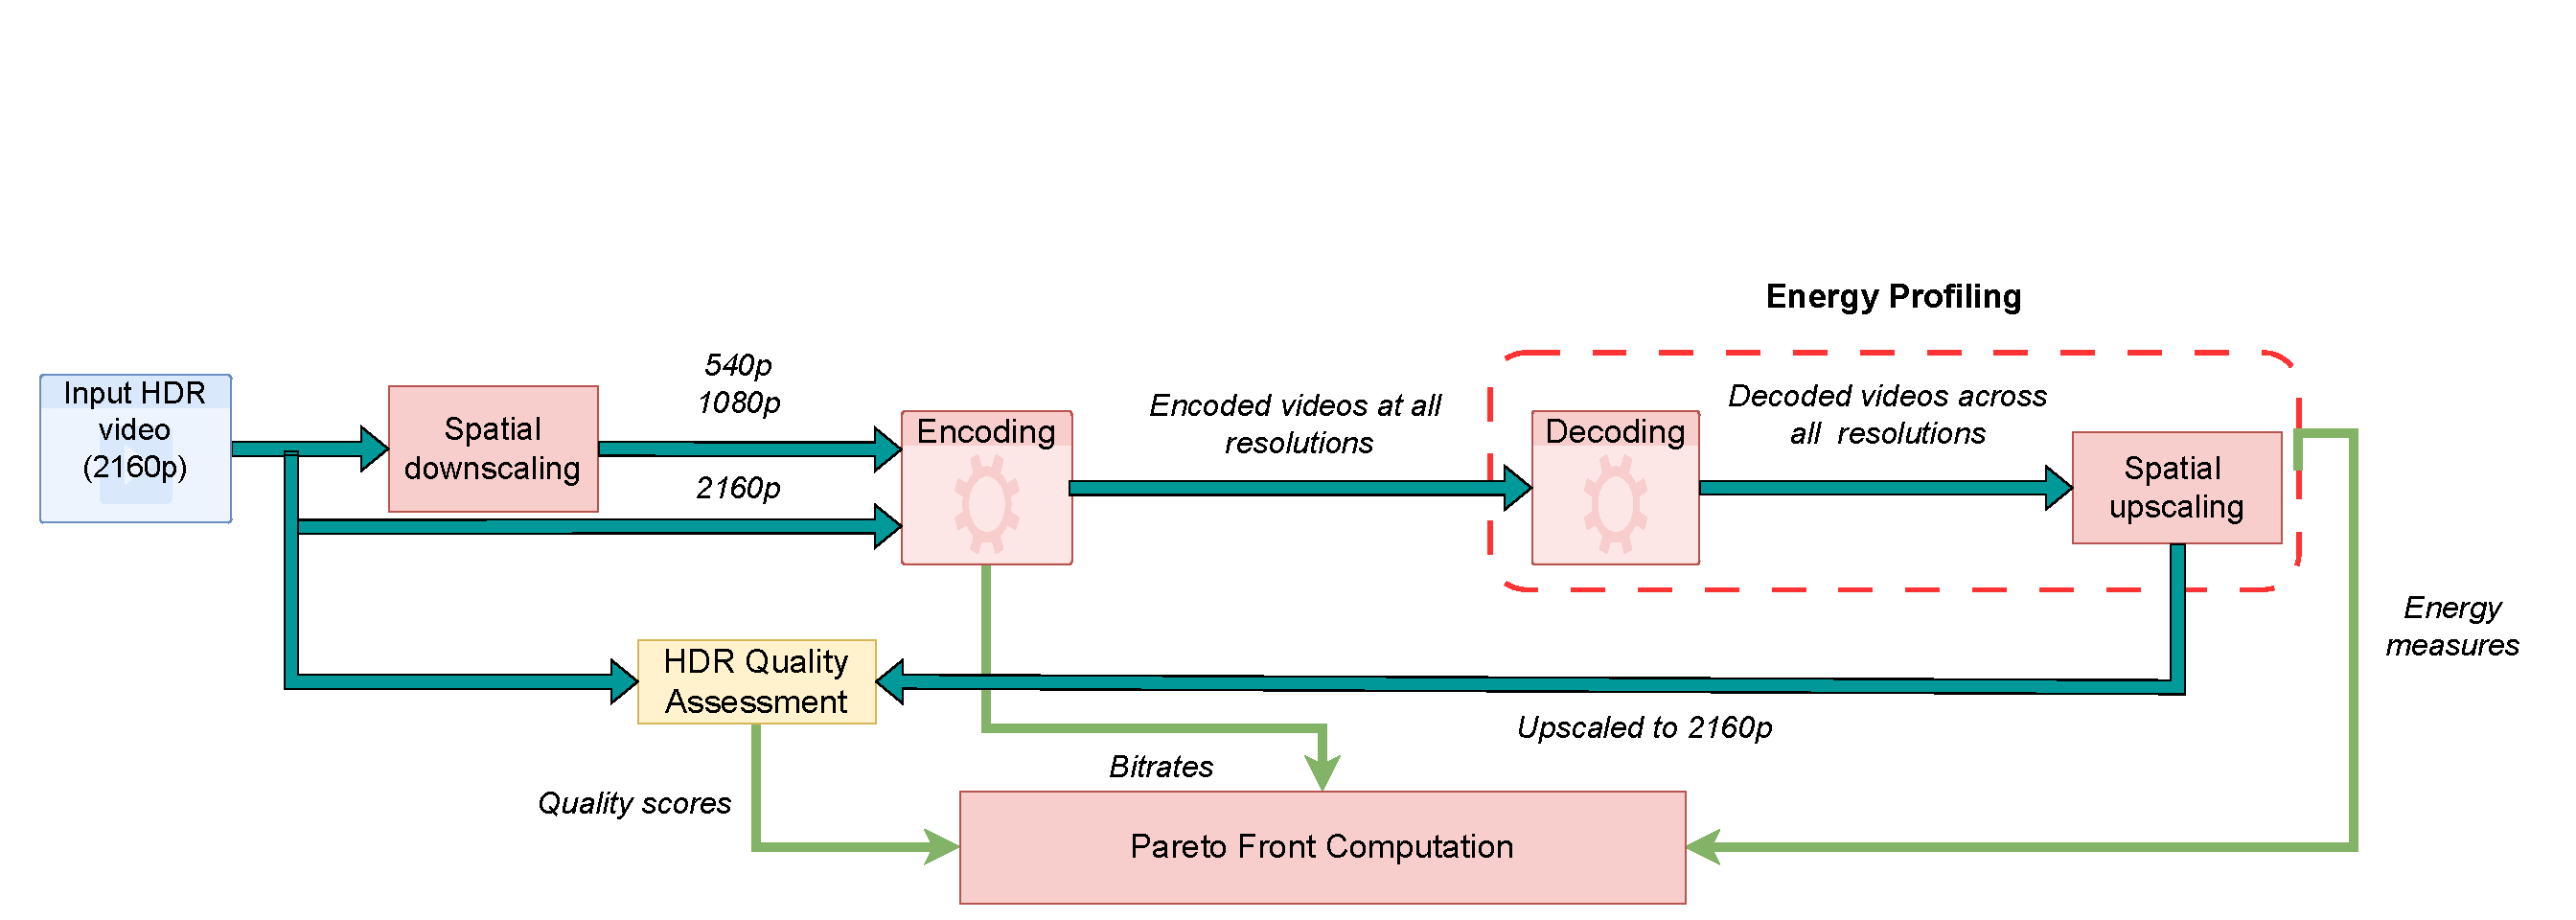
\includegraphics[width=0.89\textwidth]{Pictures/overview.pdf}
    \caption{Overview of the proposed framework.}
    \label{fig:system_overview}
\end{figure}
% Chapter Template

\chapter{Evaluation Setup}\doublespacing % Main chapter title

\label{Chapter6}

\lhead{Chapter V. \emph{Evaluation Setup}}

\setstretch{1.2}

\begin{table}[t]
\caption{Experimental parameters used in this thesis.}
\centering
\resizebox{0.575\linewidth}{!}{
\begin{tabular}{l|c|c|c|c|c|c|c}
\specialrule{.12em}{.05em}{.05em}
\specialrule{.12em}{.05em}{.05em}
\multicolumn{2}{c|}{\emph{Parameter}} & \multicolumn{6}{c}{\emph{Values}}\\
%Representation ID & 01 & 02 & 03 & 04 & 05 & 06 & 07 & 08 & 09 \\
\specialrule{.12em}{.05em}{.05em}
\specialrule{.12em}{.05em}{.05em}
\multirow{4}{*}{$\mathcal{R}$} & \emph{r [pixels]} & 360 & 432 & 540 & 540 & 540 & 720 \\
& \emph{b [Mbps]} &  0.145 & 0.300 & 0.600 & 0.900 & 1.600 & 2.400 \\
\cmidrule(lr){2-8}
& \emph{r [pixels]} & 720 & 1080 & 1080 & 1440 & 2160 & 2160 \\
& \emph{b [Mbps]} &  3.400 & 4.500 & 5.800 & 8.100 & 11.600 & 16.800\\
\hline
\multicolumn{2}{c|}{$\mathcal{C}$} & \multicolumn{6}{c}{\{YUV420, YUV422, YUV444 \} } \\
\hline
\multicolumn{2}{c|}{$\mathcal{D}$} & \multicolumn{6}{c}{8, 10}\\
\hline
\multicolumn{2}{c|}{\emph{Encoder}} & \multicolumn{6}{c}{\emph{x265 v3.6 [veryslow]}}\\
\hline
\multicolumn{2}{c|}{\emph{Decoder}} & \multicolumn{6}{c}{\emph{HM}}\\
\specialrule{.12em}{.05em}{.05em}
\specialrule{.12em}{.05em}{.05em}
\end{tabular}
}
\label{tab:exp_par}
\end{table}
 
% Chapter Template

\chapter{Experimental Results}\doublespacing % Main chapter title

\label{Chapter5}

\lhead{Chapter V. \emph{Experimental Results}}

\setstretch{1.2}

 
% Chapter Template

\chapter{Conclusions and Future Directions}\doublespacing % Main chapter title

\label{Chapter7}

\lhead{Chapter VII. \emph{Conclusions and Future Directions}} 

\section{Contributions}

\section{Limitations}

\section{Future directions}
 

%\break
%\clearpage % Start a new page
%\thispagestyle{plain}

%\addtotoc{Scope for Future Work} % Add the "Scope for future work" page entry to the Contents

%{\addtocontents{toc}{\vspace{1em}} % Add a gap in the Contents, for aesthetics
%\lhead{\emph{Scope for Future Work}} 

%\centerline{\huge \textit{{Scope for Future Work}}}
%\vspace{3em}
%In this thesis, we have worked on...

%It is hoped this work will provide the required impetus to a lot of future %study.

%}

%\clearpage % Start a new page
%----------------------------------------------------------------------------------------
%	THESIS CONTENT - APPENDICES
%----------------------------------------------------------------------------------------


\addtocontents{toc}{\vspace{2em}} % Add a gap in the Contents, for aesthetics

\appendix % Cue to tell LaTeX that the following 'chapters' are Appendices

% Include the appendices of the thesis as separate files from the Appendices folder
% Uncomment the lines as you write the Appendices

% Appendix Template

\chapter{APPENDIX CHAPTER TITLE} % Main appendix title

\label{AppendixA} % Change X to a consecutive letter; for referencing this appendix elsewhere, use \ref{AppendixX}

\lhead{Appendix A. \emph{APPENDIX CHAPTER TITLE}} % Change X to a consecutive letter; this is for the header on each page - perhaps a shortened title


Write your Appendix content here.


%% Appendix Template

\chapter{APPENDIX CHAPTER TITLE} % Main appendix title

\label{AppendixB} % Change X to a consecutive letter; for referencing this appendix elsewhere, use \ref{AppendixX}

\lhead{Appendix B. \emph{APPENDIX CHAPTER TITLE}} % Change X to a consecutive letter; this is for the header on each page - perhaps a shortened title


%% Appendix Template

\chapter{APPENDIX CHAPTER TITLE} % Main appendix title

\label{AppendixC} % Change X to a consecutive letter; for referencing this appendix elsewhere, use \ref{AppendixX}

\lhead{Appendix C. \emph{APPENDIX CHAPTER TITLE}} % Change X to a consecutive letter; this is for the header on each page - perhaps a shortened title


%\input{Appendices/AppendixD}

\addtocontents{toc}{\vspace{2em}} % Add a gap in the Contents, for aesthetics

\backmatter

%----------------------------------------------------------------------------------------
%	BIBLIOGRAPHY
%----------------------------------------------------------------------------------------
\nocite{*}
\label{References}

\lhead{\emph{Bibliography}} % Change the page header to say 
\renewcommand\bibname{Bibliography}
\bibliographystyle{IEEEtran} % Use the "custom" BibTeX style for formatting the Bibliography
%\setcitestyle{authoryear,open={((},close={))}}
{\linespread{0.8}\selectfont\bibliography{references}}



\end{document}  
